\documentclass[portrait,plainboxedsections]{sciposter}

\usepackage{amsmath}
\usepackage{amssymb}
\usepackage{multicol}
\usepackage{booktabs}
\usepackage{graphicx}
\usepackage{microtype}

\newcommand{\earlywarning}{early-warning}
\newcommand{\GW}{{\sc gw}}
\newcommand{\EM}{{\sc em}}
\newcommand{\GRB}{{\sc grb}}
\newcommand{\CBC}{{\sc cbc}}
\newcommand{\LIGO}{{\sc ligo}}
\newcommand{\LCGT}{{\sc lcgt}}
\newcommand{\GEO}{{\sc geo600}}
\newcommand{\ISCO}{{\sc isco}}
\newcommand{\SNR}{{\sc snr}}
\newcommand{\realtime}{real-time}
\newcommand{\Msun}{\ensuremath{M_{\odot}}}
\newcommand{\order}[1]{\ensuremath{\mathcal{O}[#1]}}
\newcommand{\tmpsamps}{\ensuremath{N}}
\newcommand{\numtmps}{\ensuremath{M}}
\newcommand{\numslices}{\ensuremath{S}}
% macros for number of svd basis functions
\newcommand{\SVD}{{\sc svd}}
\newcommand{\svdtmps}[1]{\ensuremath{L^#1}}
\newcommand{\numsvdtmps}{\svdtmps{s}}
% macros for sample points in slices
\newcommand{\slicesamps}[1]{\ensuremath{N^#1}}
\newcommand{\slicessamps}{\slicesamps{s}}
\newcommand{\fftblock}{\ensuremath{D}}
\newcommand{\resampsamps}{\ensuremath{N^\shortdownarrow,\, N^\shortuparrow}}
\newcommand{\fir}{{\sc fir}}
\newcommand{\fft}{{\sc fft}}
\newcommand{\fmax}{\ensuremath{f^0}}
\newcommand{\flops}{flop/s}
\newcommand{\gstlal}{{\tt gstlal}}
\newcommand{\gstreamer}{{\tt GStreamer}}
\newcommand{\numcpus}{{600}}
\newcommand{\lloid}{{\sc lloid}}
\newcommand{\TD}{{\sc td}}
\newcommand{\FD}{{\sc fd}}

% Macros for collapsing sizes of things
% From TUGboat, Volume 22 (2001), No. 4
% http://www.tug.org/TUGboat/tb22-4/tb72perlS.pdf
\def\clap#1{\hbox to 0pt{\hss#1\hss}}
\def\mathllap{\mathpalette\mathllapinternal}
\def\mathrlap{\mathpalette\mathrlapinternal}
\def\mathclap{\mathpalette\mathclapinternal}
\def\mathllapinternal#1#2{\llap{$\mathsurround=0pt#1{#2}$}} 
\def\mathrlapinternal#1#2{\rlap{$\mathsurround=0pt#1{#2}$}} 
\def\mathclapinternal#1#2{\clap{$\mathsurround=0pt#1{#2}$}}

% Colors for signal flow diagram and equation
\def\diagramcolorfir{red}
\def\diagramcolorreconstruct{blue}
\def\diagramcoloraccum{red!50!yellow}

% customize colors
\definecolor{BoxCol}{RGB}{0,35,102} % RoyalBlue
\definecolor{SectionCol}{RGB}{255,255,255} % White


\title{Toward early-warning detection of compact binary coalescence}

\author{\textsc{Nickolas V. Fotopoulos}, Leo Singer}

\institute{LIGO Laboratory, California Institute of Technology}

\email{foton@caltech.edu}

\begin{document}
\conference{Amaldi 9, Cardiff, Wales, UK; This document bears the DCC number LIGO-G1100683-v1.}

\maketitle

\begin{multicols}{3}

\section{Motivation}

\PARstart{G}{ravitational waves} are generated in the most violent events in
the history of the Universe. Stochastic gravitational-wave backgrounds (SGWBs)
can arise from both cosmological and astrophysical sources.
A cosmological SGWB can be generated from the rapid Hubble expansion of small
inhomogeneities in density, from cosmological phase transitions, and from
cosmic string cusps. The cosmological background is highly analogous to the
cosmic microwave background, but allows us to see far further back in time.
Astrophysical backgrounds arise from collections of many gravitational-wave
emitters that are too far to be resolved independently but combine incoherently
to give an appreciable signal.
%
\begin{figure}[h]
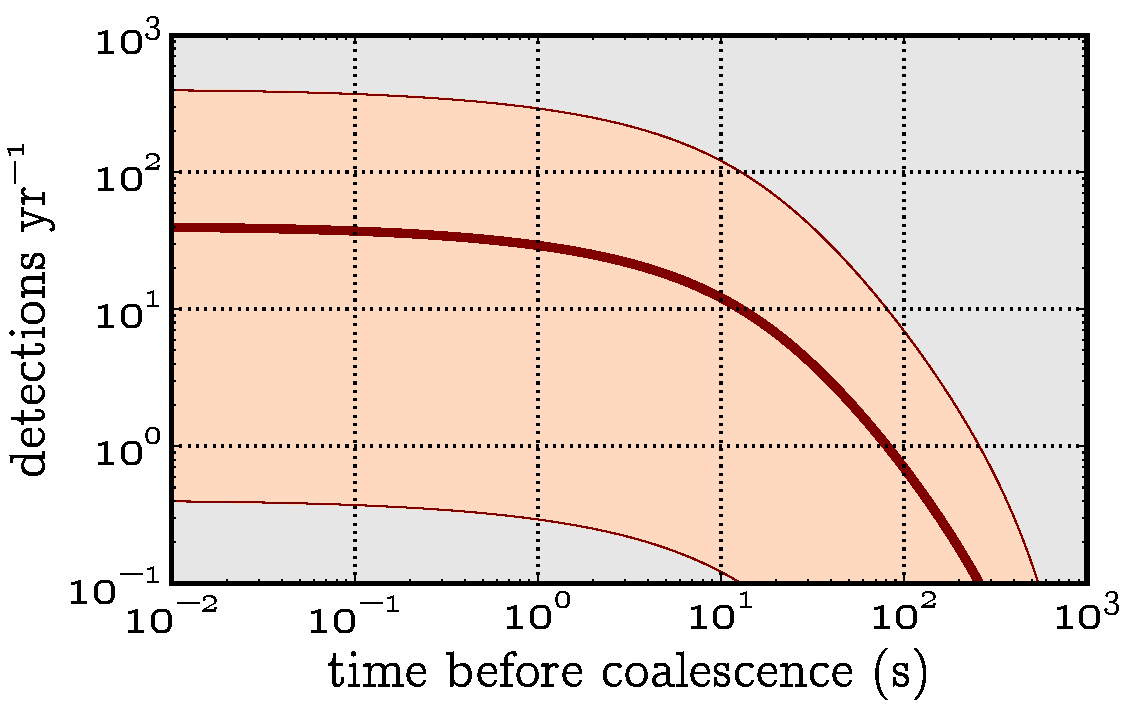
\includegraphics{figures/snr_in_time}
\caption{\label{fig:earlywarning}Expected number of \textsc{ns}--\textsc{ns}
sources that could be detectable by Advanced \LIGO\ a given number of seconds
before coalescence.  The heavy solid line is the most realistic yearly rate
estimate.  The shaded region represents the 5 to 95\% confidence interval
arising from uncertainty in predicted event rates \cite{Abadie:2010p10836}.}
\end{figure}
%
\begin{figure}[h]
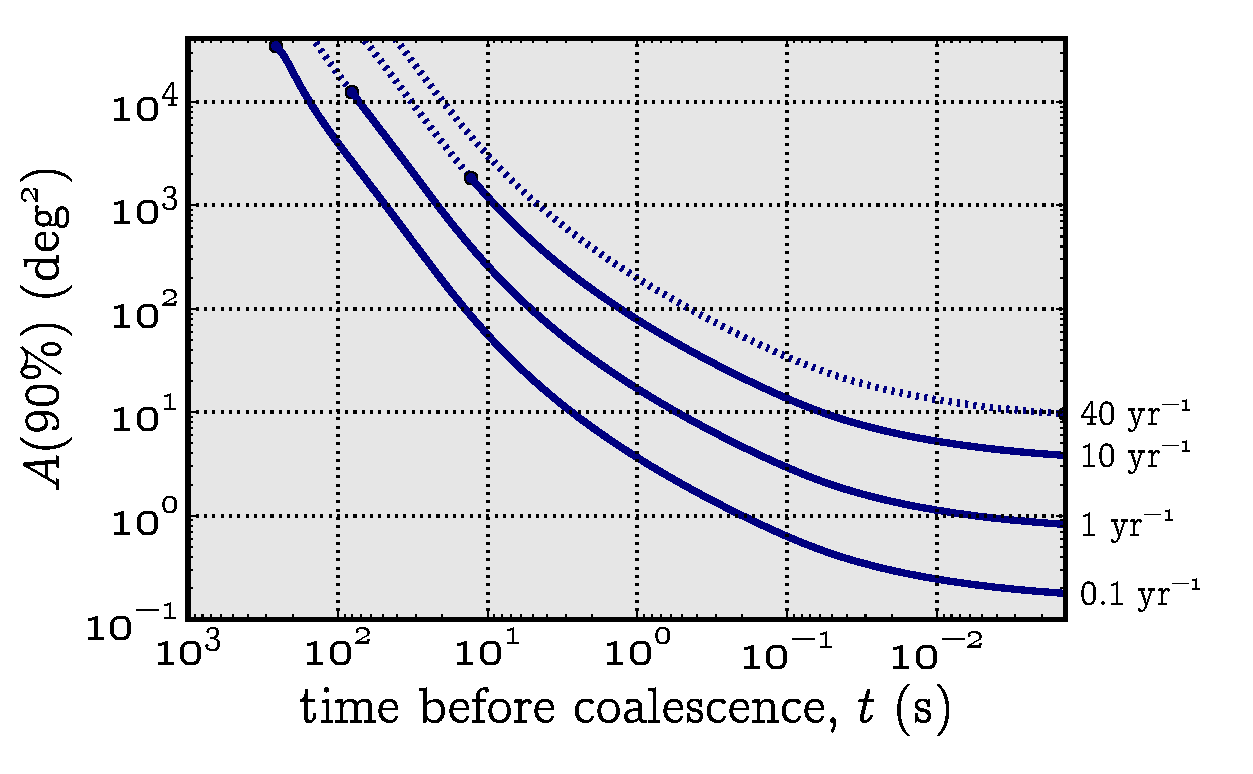
\includegraphics{figures/loc_in_time}
\caption{\label{fig:sky-localization-accuracy}Area of the 90\% confidence
region as a function of time before coalescence for sources with anticipated
detectability rates of 40, 10, 1, and 0.1~yr$^{-1}$. The heavy dot indicates
the time at which the accumulated \SNR\ exceeds a threshold of~8.}
\end{figure}

In its S5 science run, LIGO (The Laser Inteferometer Gravitational-wave
Observatory) set bounds on the combined SGWB below that set from
big-bang nucleosynthesis and today's observed elemental abundances
\cite{S5HLiso}. Advanced LIGO is expected to probe another order of
magnitude deeper.

For SGWB searches, the optimal strategy is to cross-correlate pairs of
detectors. Unavoidably, these searches incur a geometric penalty for
detectors that are separated in space and orientation. This is encoded in the
\emph{overlap reduction function}, shown in figure~\ref{f:orf}. It couples into
measurement uncertainty as $\sigma^2 \propto \int \gamma^2(|f|) \, df$
\cite{allenromano}. The uniquely co-located Hanford detectors, H1 and H2, have
an enormous geometric advantage; the advantage integrates to a factor of 10
over the Initial LIGO sensitive frequency band and a factor of 2 over the
Advanced LIGO sensitivy frequency band.

\begin{figure}
%\includegraphics{olapredfcn}
%\put(-450,350){\huge Placeholder}
\caption{Latency time-line}
\label{f:latency_timeline}
\end{figure}

\columnbreak

\begin{figure*}[h!]
	\begin{center}
		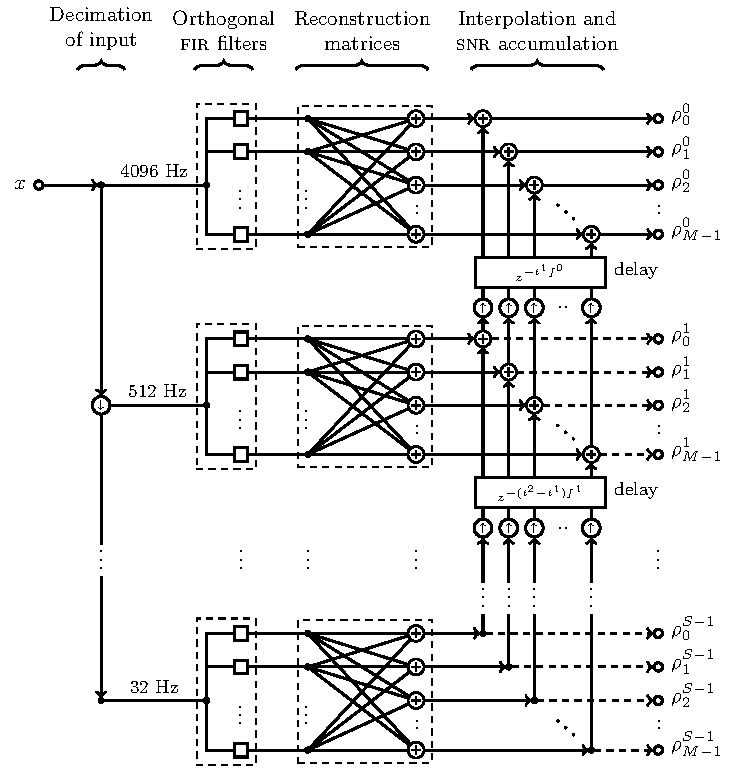
\includegraphics{figures/lloid-diagram}
		\caption{\label{fig:pipeline} Schematic of \lloid{} pipeline illustrating
signal flow.  Circles with arrows represent interpolation
\protect
\includegraphics{figures/upsample-symbol} or decimation
\protect
\includegraphics{figures/downsample-symbol}.  Circles with plus
signs represent summing junctions
\protect
\includegraphics{figures/adder-symbol}.  Squares
\protect
\includegraphics{figures/fir-symbol} stand for \fir{} filters.  Sample
rate decreases from the top of the diagram to the bottom.  In this diagram each
time slice contains three \fir\ filters that are linearly combined to produce
four output channels.  In a typical pipeline the number of \fir\ filters is
much less than the number of output channels.}
	\end{center}
\end{figure*}

\begin{multline}
	\rho_i^s [k] =%
		% Interpolation SNR
		\overbrace{
			\left(H^\uparrow \rho_i^{s+1}\right)[k]
		}^\textrm{\clap{{\sc snr} from previous time slices}} \\
		% Plus ...
		+
		% Reconstruction
		\underbrace{
			\sum_{\mathclap{l=0}}^{\mathclap{L^s-1}} v_{il}^s \sigma_l^s
		}_\textrm{\clap{reconstruction}}
		% Orthogonal FIR filter
		\overbrace{
			\sum_{\mathclap{n=0}}^{\mathclap{N^s-1}} u_l^s[n] x^s[k-n]
		}^\textrm{\clap{orthogonal {\sc fir} filters}} .
\end{multline}

\PARstart{C}{orrelations} between the H1 and H2 data streams prevent us from
fully realizing the factor of 10 advantage promised. H1 and H2 share the same
vacuum system and their optics live in the same buildings, immersing them in
a common, noisy environment. This common noise mimics the cross-correlation
signal of a SGWB.

\columnbreak

\section{Implementation}

\begin{figure}[h]
	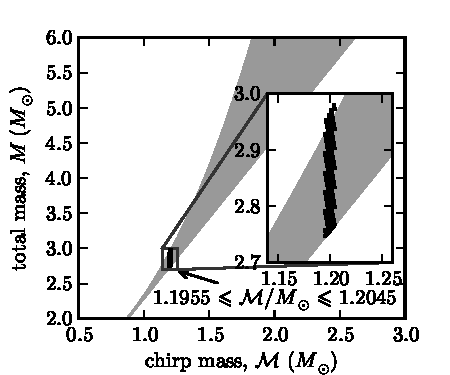
\includegraphics{figures/tmpltbank}
	\caption{\label{fig:tmpltbank}Source parameters selected for sub-bank used in this
case study, consisting of component masses $m_1$, $m_2$, between 1 and 3~$M_\odot$, and
chirp masses $\mathcal{M}$ between 1.1955 and 1.2045~$M_\odot$.}
\end{figure}

\begin{figure}
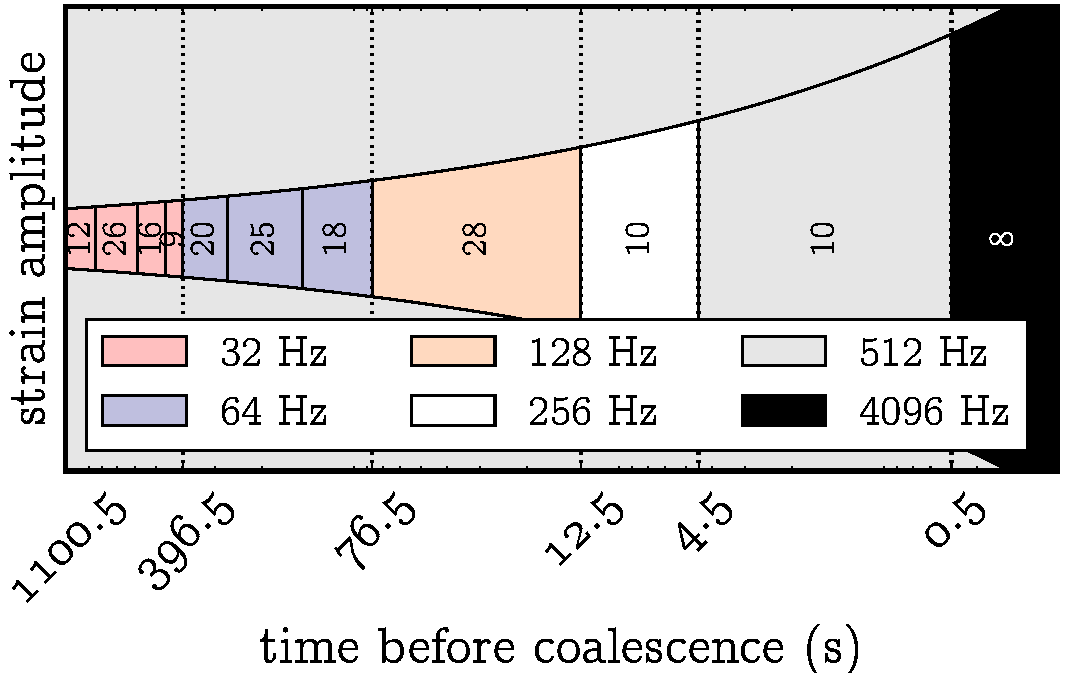
\includegraphics{figures/envelope}
\caption{envelope}
\end{figure}

\begin{table}
\begin{tabular}{rr@{,\,}lcc}
\toprule
\\ [-2ex]
$f^s$ & $[t^s$&$t^{s+1})$ & & \\% [1ex]
\\[-2.5ex]
(Hz) & \multicolumn{2}{c}{(s)} & $N^s$ & $L^s$ \\ \midrule
4096 & [0&0.5) & 2048 & 8 \\
512 & [0.5&4.5) & 2048 & 10 \\
256 & [4.5&12.5) & 2048 & 10 \\
128 & [12.5&76.5) & 8192 & 28 \\
64 & [76.5&140.5) & 4096 & 18 \\
64 & [140.5&268.5) & 8192 & 25 \\
64 & [268.5&396.5) & 8192 & 20 \\
32 & [396.5&460.5) & 2048 & 9 \\
32 & [460.5&588.5) & 4096 & 16 \\
32 & [588.5&844.5) & 8192 & 26 \\
32 & [844.5&1100.5) & 8192 & 12 \\
\bottomrule
\end{tabular}
\caption{\label{tab:time_slices} Filter design sub-bank of 657 templates.  From left to right, this table shows the sample rate, time interval, number of samples, and number of orthogonal templates for each time slice.  We vary \SVD{} tolerance from $\left(1-10^{-1}\right)$ to $\left(1-10^{-6}\right)$.}
\end{table}


\begin{figure}
\centering
%\includegraphics{olapredfcn}
%\put(-450,350){\huge Placeholder}
%\includegraphics{likelihoods}
\caption{Gstreamer pipeline.}
\label{f:gstreamer_pipeline}
\end{figure}

\section{Acknowledgements}

\LIGO\ was constructed by the California Institute of Technology and
Massachusetts Institute of Technology with funding from the National Science
Foundation and operates under cooperative agreement
\textsc{phy}-\oldstylenums{0107417}. This research
is supported by the National Science Foundation through a Graduate Research
Fellowship to LS.

%%% References

\bibliographystyle{plain}
\bibliography{biblio}

\end{multicols}

\end{document}

